\section{Redox-Reaktionen}

\subsection{Grundlagen}
    Eine Reaktion ist eine Redox-Reaktion, wenn die Oxidationszahlen der Atome der Edukte nicht die selben sind wie die Oxidationszahlen der Atome der Produkte.
    \begin{center}
        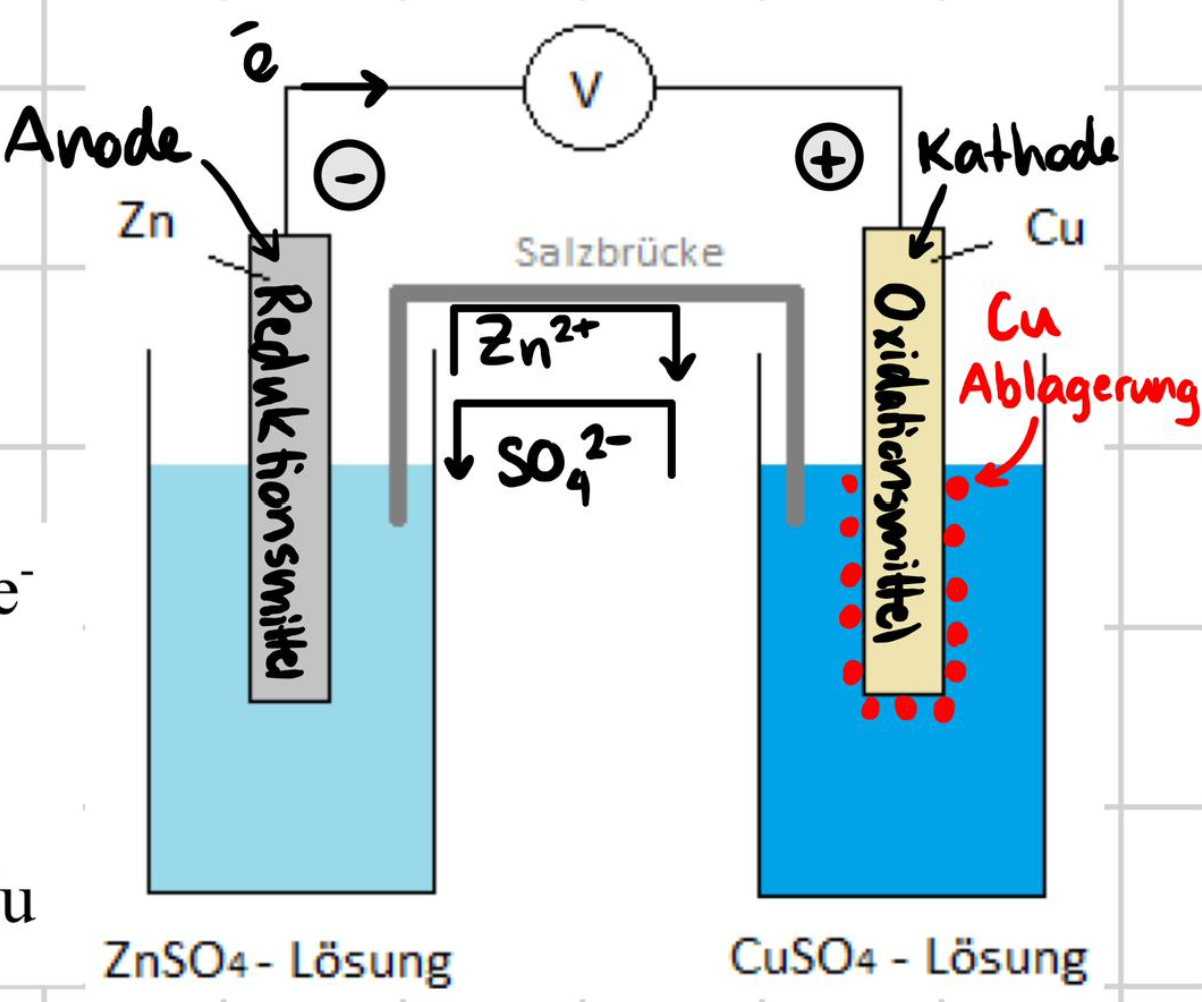
\includegraphics[height=4cm]{pictures/Galv.png}
    \end{center}
    Aufgrund der \textbf{Standartpotenziale} der Metalle Zn und Cu herrscht eine ``Spannun'', welche die Reaktion ermöglicht. 
    Das \textbf{\ce{Zn^0}} wird an der Anode zu \textbf{\ce{Zn^2+}} oxidiert (\ce{e^-}-Abgabe), \textbf{\ce{Zn^0}} dient somit als Reduktionsmittel. 
    Die Elektronen werden an die Kathode abgegeben, wo \textbf{\ce{Cu^2+}} aus der Lösung zu \textbf{\ce{Cu^0}} reduziert (\ce{e^-}-Aufnahme) wird. 
    \textbf{\ce{Cu^2+}} dient somit als Oxidationsmittel. Damit die Lösungen jeweils ungeladen bleiben, wandern über die Salzbrücke 
    \textbf{\ce{Zn^2+}-Ionen} und \textbf{\ce{SO4^2-}-Ionen}.
\subsection{Redoxpotential}
    Das Redoxpotential einer Halbzelle kann aus der Redox-Reihe ausgelesen werden (ganz rechts). Dieses Potenzial wurde jeweils 
    gegenüber einer Standart-Wasserstoff-Elektrode gemessen.
    
    Das Redoxpotential ist jedoch von pH, Druck, Ionenkonz und Temperatur abhängig. Potenziale bei Nicht-Standardbedingungen können 
    mit folgender GLeichung berechnet werden.

    Nernst-Gleichung:\\
    \begin{minipage}{0.4\linewidth}
        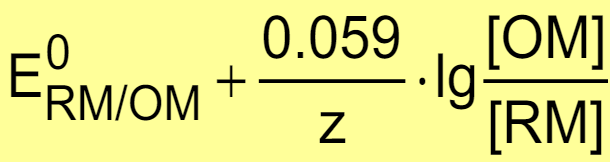
\includegraphics[width=\linewidth]{pictures/Nernst.png}
    \end{minipage}
    \hfill
    \begin{minipage}{0.55\linewidth}
        \begin{itemize}
            \item z = Anz. \ce{e^-} die pro Atom übergeben werden
            \item \ce{[OM]} = konz. OM in mol/L
            \item \ce{[RM]} = konz. RM in mol/L
        \end{itemize}
    \end{minipage}

    \begin{center}
        Inkl. pH-Wert:\\
        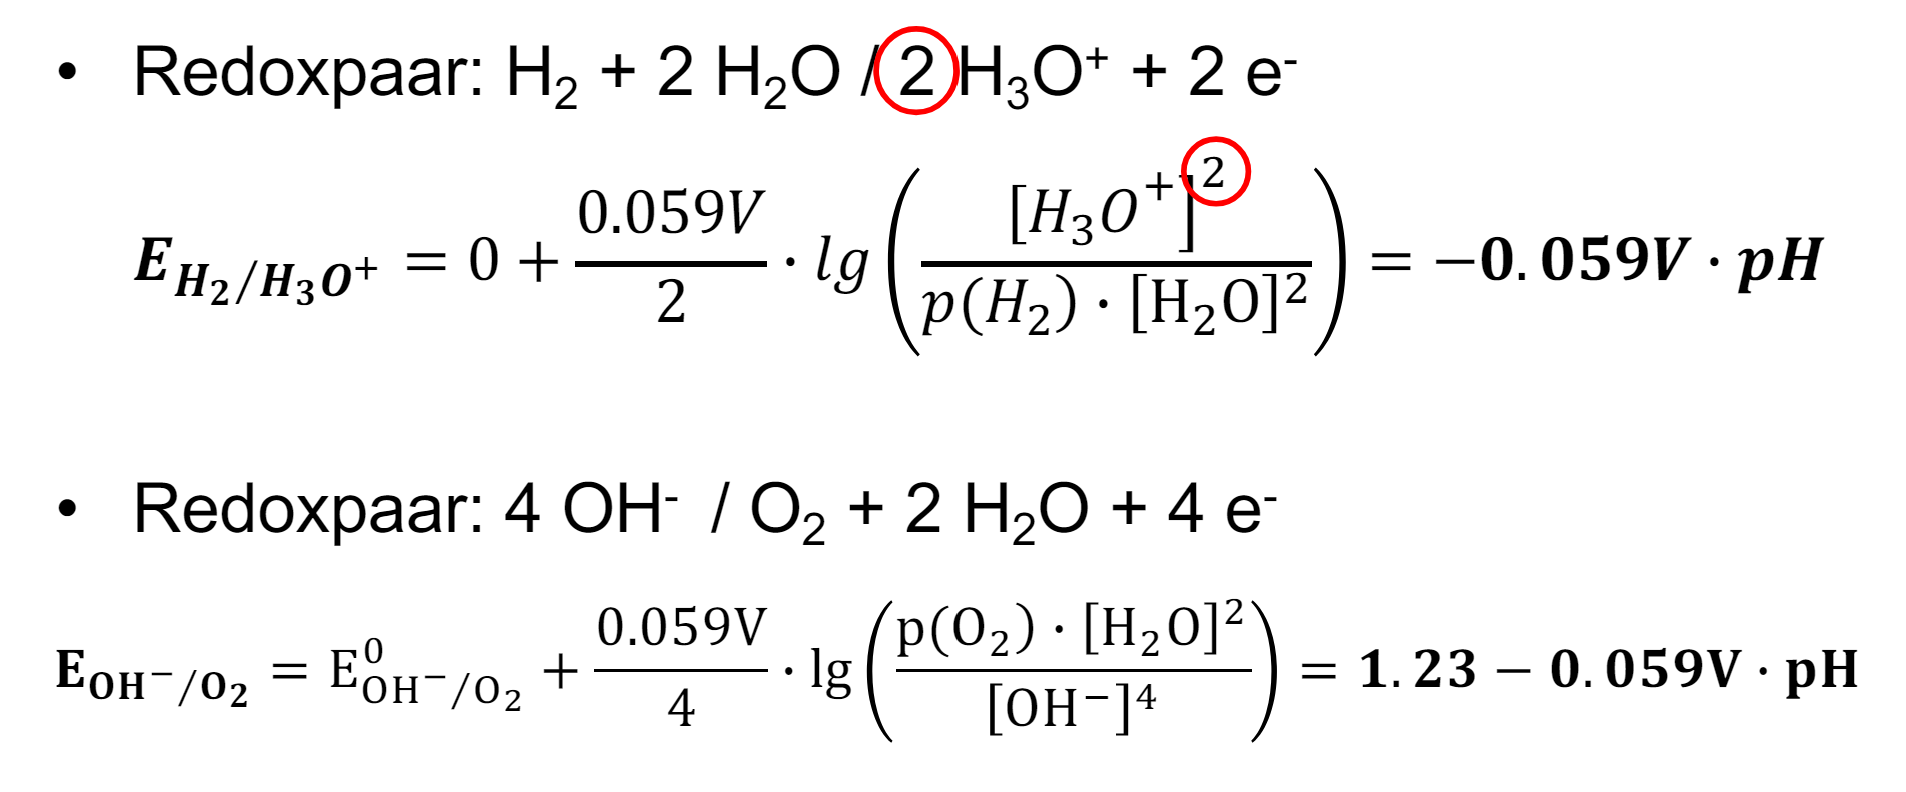
\includegraphics[height=3cm]{pictures/Nernstph.png}
    \end{center}